\section{Prerequisites}

\subsection{Homogenous Coordinates} \label{sec:homogenous}

While Euclidean space describes 2D and 3D space well, they are not sufficient in describing perspective projections.


Homogenous coordinates (also known as projective coordinates)

When
(u,v)


In other words, with homogenous coordinates, we interpret our \emph{Euclidean} space as an \emph{affine} space

\begin{figure}[H]
    \centering
    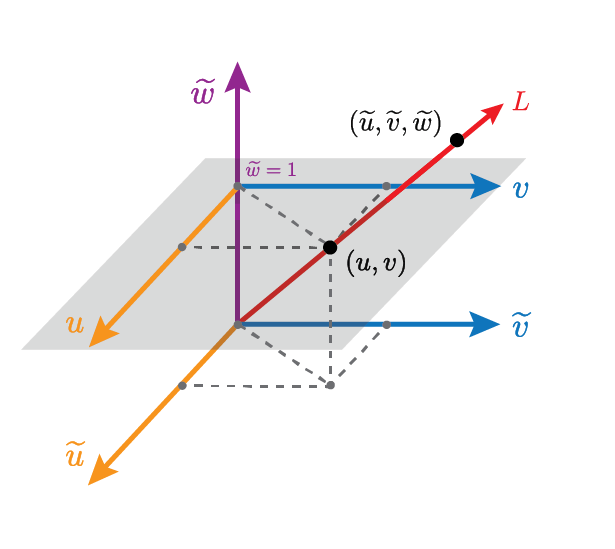
\includegraphics[width=0.6\textwidth]{figures/homogenous}
    \caption{Homogenous coordinate system.}
\end{figure}
